% !TeX root = main.tex

% Dokumenteinstellungen und Anpassungen
\documentclass[chapterprefix=false, 12pt, a4paper, oneside, parskip=half, listof=totoc, bibliography=totoc, numbers=noendperiod]{article}

%\renewcommand{\familydefault}{\sfdefault}
%\usepackage{helvet}

\usepackage[bottom=35mm,left=25mm,right=25mm]{geometry}

\usepackage{csquotes}
\usepackage[round,sort&compress, authoryear]{natbib}
\bibliographystyle{plainnat}

\usepackage{scrhack}

\usepackage{tabularx} % in the preamble

%Blindtext
\usepackage{blindtext}

\usepackage{caption}

\usepackage{imakeidx}

\usepackage{paralist}

\usepackage{epigraph}

\usepackage[toc, acronym]{glossaries}


\usepackage[automark,headsepline]{scrlayer-scrpage}
\setlength{\parindent}{0em}

\usepackage[onehalfspacing]{setspace}

\usepackage[stretch=10]{microtype}

% English language settings
\usepackage[english]{babel}

\usepackage{lmodern}
\usepackage[utf8]{inputenc}
\usepackage[T1]{fontenc}
\setlength{\emergencystretch}{1em}

\usepackage{epigraph}

\usepackage{float}

\usepackage{tabularx}

\usepackage{longtable}

\usepackage{listings}

\usepackage[table,xcdraw]{xcolor}

\usepackage{tikz}

\usepackage{graphicx}

\usepackage{wrapfig}

\usepackage[hidelinks]{hyperref}

\input{resources/styles/adjustments}

\usepackage{graphicx}
\usepackage{subcaption}
\usepackage{float}
\usepackage{color}
\usepackage{listings}
\usepackage{animate}
\usepackage{eso-pic}

\newcommand\BackgroundPic{%
\put(0,0){%
\parbox[b][\paperheight]{\paperwidth}{%
\vfill
\centering
\includegraphics[width=\paperwidth,height=\paperheight,%
keepaspectratio]{resources/images/deckblatt.png}%
\vfill
}}}

\makeatletter
\newcommand*{\germanTitle}[1]{\gdef\@germanTitle{#1}}
\newcommand*{\englishTitle}[1]{\gdef\@englishTitle{#1}}
\newcommand*{\gradeType}[1]{\gdef\@gradeType{#1}}
\newcommand*{\firstExaminer}[1]{\gdef\@firstExaminer{#1}}
\newcommand*{\secondExaminer}[1]{\gdef\@secondExaminer{#1}}
\newcommand*{\matrikelnr}[1]{\gdef\@matrikelnr{#1}}
\newcommand*{\authorBirthplace}[1]{\gdef\@authorBirthplace{#1}}
\newcommand*{\submitDate}[1]{\gdef\@submitDate{#1}}
\newcommand*{\discipline}[1]{\gdef\@discipline{#1}}
\newcommand*{\courseOfStudies}[1]{\gdef\@courseOfStudies{#1}}
\newcommand*{\authorLastname}[1]{\gdef\@authorLastname{#1}}
\newcommand*{\authorFirstname}[1]{\gdef\@authorFirstname{#1}}

\renewcommand*{\maketitle}{
	\begin{titlepage}
		\newgeometry{left=3.8cm,right=2.5cm,top=4.6cm,bottom=2.5cm}
			\begingroup
				\fontsize{32pt}{32pt}\selectfont
				{\bfseries Bachelor Thesis}
			\endgroup

			\vskip 1.44cm

			\begingroup
			\fontsize{8pt}{6pt}\selectfont
			Title of the Thesis // Titel der Arbeit
			\endgroup

			\vskip -0.02cm

			\begingroup
			\fontsize{14pt}{14pt}\selectfont
			{\bfseries \@englishTitle\par}
			\vspace{0.3cm} % Add vertical space between German and English title
			{\@germanTitle\par}
			\endgroup
			\vskip -0.1cm

			\noindent\rule{15cm}{0.4pt}
			
			\vskip 0.05cm

			\begingroup
			\fontsize{8pt}{6pt}\selectfont
			Academic Degree // Akademischer Grad
			\endgroup

			\vskip -0.15cm

			\begingroup
			\fontsize{12pt}{14pt}\selectfont
				{\@gradeType}
			\endgroup
			\vskip -0.15cm

			\noindent\rule{15cm}{0.4pt}
			
			\vskip 0.05cm

			\begingroup
			\fontsize{8pt}{6pt}\selectfont
			Author's Name, Place of Birth // Name der Autorin/des Autors, Geburtsort
			\endgroup

			\vskip -0.15cm

			\begingroup
			\fontsize{12pt}{14pt}\selectfont
				{\@authorFirstname} {\@authorLastname}, {\@authorBirthplace}
			\endgroup
			\vskip -0.15cm

			\noindent\rule{15cm}{0.4pt}
			
			\vskip 0.05cm

			\begingroup
			\fontsize{8pt}{6pt}\selectfont
			Field of Study // Studiengang
			\endgroup

			\vskip -0.15cm

			\begingroup
			\fontsize{12pt}{14pt}\selectfont
				{\@courseOfStudies}
			\endgroup
			\vskip -0.15cm

			\noindent\rule{15cm}{0.4pt}
			
			\vskip 0.05cm

			\begingroup
			\fontsize{8pt}{6pt}\selectfont
			Department // Fachbereich
			\endgroup

			\vskip -0.15cm

			\begingroup
			\fontsize{12pt}{14pt}\selectfont
				{\@discipline}
			\endgroup
			\vskip -0.15cm

			\noindent\rule{15cm}{0.4pt}
			
			\vskip 0.05cm

			\begingroup
			\fontsize{8pt}{6pt}\selectfont
			First Examiner // Erstprüferin/Erstprüfer
			\endgroup

			\vskip -0.15cm

			\begingroup
			\fontsize{12pt}{14pt}\selectfont
				{\@firstExaminer}
			\endgroup
			\vskip -0.15cm

			\noindent\rule{15cm}{0.4pt}
			
			\vskip 0.05cm

			\begingroup
			\fontsize{8pt}{6pt}\selectfont
			Second Examiner // Zweitprüferin/Zweitprüfer
			\endgroup

			\vskip -0.15cm

			\begingroup
			\fontsize{12pt}{14pt}\selectfont
				{\@secondExaminer}
			\endgroup
			\vskip -0.15cm

			\noindent\rule{15cm}{0.4pt}
			
			\vskip 0.05cm

			\begingroup
			\fontsize{8pt}{6pt}\selectfont
			Matriculation Number // Matrikelnummer
			\endgroup

			\vskip -0.15cm

			\begingroup
			\fontsize{12pt}{14pt}\selectfont
				{\@matrikelnr}
			\endgroup
			\vskip -0.15cm

			\noindent\rule{15cm}{0.4pt}

			\vskip 0.05cm

			\begingroup
			\fontsize{8pt}{6pt}\selectfont
			Date of Submission // Abgabedatum
			\endgroup

			\vskip -0.15cm

			\begingroup
			\fontsize{12pt}{14pt}\selectfont
				{\@submitDate}
			\endgroup
			\vskip -0.15cm

			\noindent\rule{15cm}{0.4pt}
		\restoregeometry
	\end{titlepage}
}
\makeatother

% Variablen für das Deckblatt
\gradeType{Bachelor of Science (B.Sc.)}
\germanTitle{Wissenschaftliche Softwareentwicklung eines Convolutional Neuronal Networks für die Rekonstruktion fehlender Daten einer Wettermessstation unter Verwendung von Numerischen Modelldaten}
\englishTitle{Scientific software development of a Convolutional Neural Network for the reconstruction of missing data from a weather measurement station using numerical model data.}
\authorFirstname{Timo}
\authorLastname{Wacke}
\authorBirthplace{Hamburg}
\discipline{Computer Science // Informatik}
\courseOfStudies{Computing in Science (Physics Specialization)}
\matrikelnr{7434883}
\submitDate{10.06.2024}
\firstExaminer{Prof. Dr. Thomas Ludwig}
\secondExaminer{Dr. Christopher Kadow}


\makeatletter

\newcommand*{\place}[1]{\gdef\@place{#1}}

\newcommand*{\makeeidesstatt}{
	\begin{titlepage}
		\newgeometry{left=3.8cm,right=2.5cm,top=8cm,bottom=2.5cm}
			\begingroup
			\fontsize{18pt}{20pt}\selectfont
			{\bfseries Eidesstattliche Versicherung}
			\endgroup

			\vskip 0.8cm

			\begingroup
			\fontsize{12pt}{14pt}\selectfont
				{\@authorLastname} {\@authorFirstname}
			\endgroup

			\vskip -0.5cm

			\noindent\rule{15cm}{0.4pt}

			\vskip -0.4cm

			\begingroup
			\fontsize{8pt}{6pt}\selectfont
			Last Name, First Name // Name, Vorname
			\endgroup

			\vskip 0.6cm
			\begingroup
			\fontsize{10.5pt}{11.5pt}\selectfont
   
			„Hiermit versichere ich an Eides statt, dass ich die vorliegende Arbeit mit dem Titel
			\endgroup

			\begingroup
			\fontsize{16pt}{18pt}\selectfont
			{\bfseries \@germanTitle}
			\endgroup

			\begingroup
			\fontsize{10.5pt}{11.5pt}\selectfont
			im Bachelorstudiengang \@courseOfStudies selbstständig verfasst und keine anderen als die angegebenen Hilfsmittel – insbesondere keine im Quellenverzeichnis nicht benannten Internet-Quellen – benutzt habe. Alle Stellen, die wörtlich oder sinngemäß aus Veröffentlichungen entnommen wurden, sind als solche kenntlich gemacht. Ich versichere weiterhin, dass ich die Arbeit vorher nicht in einem anderen Prüfungsverfahren eingereicht habe.
			\endgroup

			\vskip 0.8cm

			{
			\fontsize{12pt}{14pt}\selectfont
			{\@place}, den {\today}
			}

			\vskip -0.5cm

			\noindent\rule{15cm}{0.4pt}

			\vskip -0.3cm

			\begingroup
			\fontsize{8pt}{6pt}\selectfont
			Place, Date, Signature // Ort, Datum, Unterschrift
			\endgroup


		\restoregeometry
	\end{titlepage}}
\makeatother

\place{Hamburg}


\lstset{literate=%
  {Ö}{{\"O}}1
  {Ä}{{\"A}}1
  {Ü}{{\"U}}1
  {ß}{{\ss}}1
  {ü}{{\"u}}1
  {ä}{{\"a}}1
  {ö}{{\"o}}1
}

% Javascript als Sprache für die lstings
\lstdefinelanguage{JavaScript}{
  keywords={typeof, new, true, false, catch, function, return, null, catch, switch, var, if, in, while, do, else, case, break, that, globals, let, const},
  keywordstyle=\color{blue}\bfseries,
  ndkeywords={class, export, boolean, throw, implements, import, this},
  ndkeywordstyle=\color{darkgray}\bfseries,
  identifierstyle=\color{black},
  sensitive=false,
  comment=[l]{//},
  morecomment=[s]{/*}{*/},
  commentstyle=\color{gray}\ttfamily,
  stringstyle=\color{red}\ttfamily,
  morestring=[b]',
  morestring=[b]"
}
\lstset{
    language=JavaScript,
    numbers=none,
    frame=leftline,
    tabsize=2,
    rulesepcolor=\color{gray},
    rulecolor=\color{black},
    captionpos=b,
    breaklines=true,
    breakatwhitespace=false,
}

\lstdefinelanguage{Python}{
    keywords={self, def, class, import, from, if, else, elif, for, while, return, True, False, None},
    keywordstyle=\color{blue}\bfseries,
    ndkeywords={},
    ndkeywordstyle=\color{darkgray}\bfseries,
    identifierstyle=\color{black},
    sensitive=true,
    comment=[l]{\#},
    morecomment=[s]{"""}{"""},
    commentstyle=\color{gray}\ttfamily,
    stringstyle=\color{orange}\ttfamily,
    morestring=[b]',
    morestring=[b]"
}

\lstset{
    language=Python,
    numbers=left,            % Line numbers on the left side
    tabsize=2,
    captionpos=b,
    breaklines=true,
    breakatwhitespace=false,
}

\newcommand{\subsubsubsection}[1]{\paragraph{#1}\mbox{}\\}
\setcounter{secnumdepth}{4}
\setcounter{tocdepth}{4}
\begin{document}

% Entfernen der Seitenzahlen und BackroundPic als Hintergrund nutzen
\pagenumbering{gobble}
\AddToShipoutPicture{\BackgroundPic}

% Titelblatt erzeugen
\maketitle
\newpage

% Eidesstattliche Erklärung erzeugen
\makeeidesstatt
\thispagestyle{empty}

% Abstract und Inhaltsverzeichnisse einfügen (Numerierung römisch ab Inhaltsverzeichnis)
\section*{Abstract}
\label{sec: abstract}

This bachelor thesis develops and presents a deep learning technique to reconstruct missing 2-meter temperature measurements of weather stations.
By supporting low-cost 3D printed stations with gap-filling, this thesis addresses challenges posed by sparse weather station coverage.
The proposed method involves a supervised training of a convolutional neural network to estimate weather station's hourly measurements solely based on the surrounding 8x8 grid or \textasciitilde 250x250km temperature data from the ERA5 Reanalysis by the European Centre of Medium-Range Weather Forecast.
The trained model demonstrates the capacity to reconstruct missing station data with a computational efficiency that surpasses that of traditional numerical models.
The thesis describes the conceptual framework and its transition to an applied framework, including data acquisition, preprocessing, neural network training, and model validation for infilling.
A model was trained and validated for three weather stations in mountain, ocean, and city terrain. The model was tested using a root mean square error and Pearson correlation coefficient over various time dimensions.
The results demonstrated a reduction in errors and an increase in correlation upon the input data ERA5, despite limited training data availability in some cases. To facilitate the application of the method, an end-to-end software solution was developed, including a user-friendly web interface.
This flexible approach enables users to train, validate, and apply models to any other station beyond the scope of this thesis.
In conclusion, this thesis not only presents a novel deep learning approach for reconstructing missing temperature measurements, but also provides a practical, scalable solution for enhancing the reliability of low-cost weather stations worldwide.

\newpage

\section*{Zusammenfassung}

Diese Bachelorarbeit entwickelt und präsentiert eine Deep-Learning-Technik zur Rekonstruktion fehlender 2-Meter-Temperaturmessungen von Wetterstationen.
Und unterstützt damit Bemühungen für eine besseren Stations-Abdeckung mittels kostengünstigeren aber damit auch unverlässlicheren Wetterstationen, durch diese Arbeit unterstützt werden.
Die vorgeschlagene Methode umfasst ein überwachtes Training eines Convolutional Neural Networks, um stündliche Messungen der Wetterstationen ausschließlich auf Basis der umliegenden 8x8 Raster oder \textasciitilde 250x250 km Temperatursdaten aus der ERA5-Reanalyse des Europäischen Zentrums für mittelfristige Wettervorhersagen zu schätzen.
Das trainierte Modell kann, fehlende Stationsdaten mit einer Effizienz zu rekonstruieren, die traditionelle numerische Modelle übertrifft.
Die Arbeit beschreibt den konzeptionellen Rahmen und dessen Umsetzung in einen anwendungsorientierten Rahmen, einschließlich Datenerfassung, Datenvorverarbeitung, Training des neuronalen Netzwerks und Modellvalidierung zur Rekonstruktion.
Je ein Modell wurde für drei Wetterstationen in Berg-, Ozean- und Stadtgebieten trainiert und validiert.
Das Modell wurde mit dem Root Mean Square Error und dem Korrelationskoeffizienten über verschiedene Zeitdimensionen getestet.
Die Ergebnisse zeigten eine Reduzierung der Fehler und eine erhöhte Korrelation im Vergleich zu den Eingangsdaten aus ERA5, trotz begrenzter Verfügbarkeit von Trainingsdaten in einigen Fällen.
Um die Anwendung der Methode zu erleichtern, wurde eine End-to-End-Softwarelösung entwickelt, die eine benutzerfreundliche Weboberfläche umfasst.
Dieser flexible Ansatz ermöglicht es den Benutzern, Modelle zu trainieren, zu validieren und auf beliebige andere Stationen anzuwenden, die über den Rahmen dieser Arbeit hinausgehen.
Abschließend präsentiert diese Arbeit nicht nur einen neuartigen Deep-Learning-Ansatz zur Rekonstruktion fehlender Temperaturmessungen, sondern bietet auch eine praktische, skalierbare Lösung zur Verbesserung der Zuverlässigkeit kostengünstiger Wetterstationen weltweit.
\ClearShipoutPicture
\thispagestyle{empty}
\newpage

% Acknowledgements
\section*{Acknowledgements}

Thank you Chris
\thispagestyle{empty}
\newpage

\pagenumbering{Roman}
\tableofcontents
\newpage
\listoffigures
\newpage

% Kapitel einfügen
\pagenumbering{arabic}
\section{Introduction}
\label{sec:introduction}

% Weather stations are sparse in some regions

Weather station density varies greatly across the globe, depending on population density, economic development, and access to nearby infrastructure \cite{ortizbobea2021}.
While any weather station can experience downtime, the reliability of weather stations in regions with low station density is often low as well \cite{Mistry2022GlobalWS}.
So not only is downtime in regions where data is limited more likely, but it is also more impactful because there are fewer neighboring stations to help compensate for the missing data.

A denser, more reliable network would benefit weather forecasting, helping to evacuate populations timely before natural disasters \cite{muita2021} and would contribute globally available climate data.
An innovative approach to increase the density of weather stations could be to use low-cost weather stations that could be 3D-printed and assembled by the local population \cite{muita2021}. This is the approach taken by the 3D-PAWS project (see \autoref{sec:3d_printed_stations}).
Either way, low-cost weather stations have reliability issues and are prone to downtime. In this work, out of the many globally deployed stations of the 3D-PAWS project, three stations that have many years of history have been selected for the evaluation of the proposed method. One station is located on an island surrounded by ocean, Barbados, one in a city, Vienna, and one in a mountainous region, Boulder, Colorado. In \autoref{fig:vienna_measurements}, temperature measurements of the Vienna station since its deployment in 2017 are shown, illustrating an extreme case of downtime.

\begin{figure}
    \centering
    \includegraphics[width=0.8\textwidth]{resources/images/charts/vienna_available_measurements_bw.png}
    \caption{Temperature measurements of a 3D-printed weather station in Vienna, Austria.}
    \label{fig:vienna_measurements}
\end{figure}

% Let's connect aerial data with local measurements

In light of the challenges posed by sparse weather station coverage, novel methodologies are required to address the reconstruction of missing weather data.
Machine learning offers a promising alternative to traditional numerical reconstruction methods, such as kriging, that rely on neighboring station data and are often computationally intensive \cite{chung2019kriging}. Numerical alternatives like Weather Research and Forecasting (WRF) models provide greater accuracy than kriging but are even more computationally demanding \cite{skamarock2008wrf}.
The application of machine learning, in this case, would be to relate coarse-resolution numerical reanalysis data, which in itself can not accurately describe the local characteristics, to the local patterns at the weather station.
This would allow for independent operation without relying on neighboring stations or additional data sources. It can directly utilize the global reanalysis data as input, outperforming numerical methods in terms of computational resource requirements by orders of magnitude \cite{kurth2023MLperformance,bi2023MLperformance,lam2023MLperformance} as the application of the trained machine-learning model.
By leveraging available local data, these techniques, such as Convolutional Neural Networks (CNNs), can be trained to estimate weather conditions at a designated time by assimilating global numerical weather model data.
Despite the inherent blurriness of aerial data provided in grid cells, these models are anticipated to discern and adapt to local weather patterns such that they become capable of transferring knowledge from the meta situation to the local situation.
This paper aims to achieve reconstruction using that approach, which will be further explained in \autoref{sec: design}.

% ERA5 0.25 hourly everywhere

The reanalysis of choice in this endeavor is the ECMWF Reanalysis v5 (ERA5), which covers the globe in grid cells of 0.25° x 0.25°.
The data is available in hourly timesteps from 1940 to the present and contains a wide range of variables, such as temperature, precipitation, wind speed, and many more \cite{era5}.

% Let's go with the temperature

To prove the concept it is likely easiest to start with temperature data, meaning the 2m temperature variable from the ERA5 reanalysis will be used as input to the neural net.


\section{3D printed Weather Stations}
\label{sec:3d_printed_stations}
\section{Conceptual Framework}
\label{sec:design}

\subsection{Concept}

\begin{figure}
    \centering
    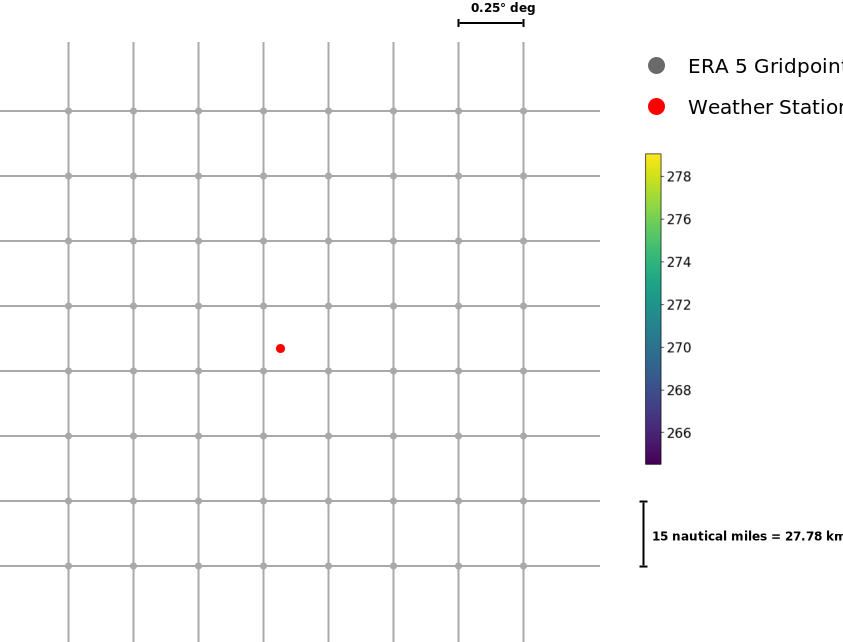
\includegraphics[width=\textwidth]{resources/images/ERA5_tas_around_barbados.png}
    \caption{8x8 grid-points of ERA5 with 2m temperature 
    for 2020-06-23 19:00 UTC  in the area of a weather station on Barbados}    
    \label{fig:barbados}
\end{figure}

\begin{figure}
    \centering
    \includegraphics[width=0.9\textwidth]{resources/images/supervised_learning.png}
    \caption{Conceptual framework using supervised learning.}
    \label{fig:supervised_learning}
\end{figure}

The conceptual framework of the proposed method is illustrated in \autoref{fig:concept}.
Applying the local patterns at the weather station location on top of ERA5 would reconstruct the temperature data at the station.
The idea is that a Convolutional Neural Network would learn to recognize the relevant patterns in a regional cutout of ERA5 data in the station area.
Based on the regional ERA5 data, the network would then predict the temperature at the weather station.
To illustrate with an example in what form these discrepancies can emerge:
In the case of Barbados, the grid cells of the ERA5 data all lay primarily in the ocean, meaning the diurnal cycle has a much lower amplitude than at the weather station that is located on land. The neural network would need to learn how to detect the diurnal cycle phase based on the 64 grid points and then adjust the temperature values accordingly. Besides this obvious difference between ERA5 and the measurements at Barbados, there are most likely many more dynamic local effects to be learned and adjusted for.

Since the ERA5 data is available globally and hourly, any weather station's missing hour could be reconstructed simply with a model that has been trained for the respective station.
To train the model, a supervised learning approach will be used.
Therefore, the model's weight will be adjusted during training so that the difference between the prediction based on an ERA5 input and the actual measurement is minimized.
The design decision to make the model based on one timestep of input for one timestep of output and not on a sequence of timesteps has following advantages: It allows for simplicity in training, as no sequence handling is needed but simply any single timestep can be used for training.
It also allows for flexibility in application, as the model can be applied to any single timestep of ERA5 data to reconstruct the temperature at the weather station at that time.
The disadvantage is that the model can not learn from the sequence of timesteps, meaning it can not learn from the temporal evolution of the weather patterns, but that is not anticipated to be a problem since all that information is already included in the ERA5 data.
Therefore, when reconstructing missing data, the model is applied to the ERA5 data hour by hour, and the result is a series of hourly predictions that are not connected in time.

% In \autoref{fig:barbados} ERA5 grid points around a weather station on Barbados are shown along with their corresponding temperature two meters above the surface. The graph is for the hour 19:00 UTC on the 23rd of June 2020. Along the latitude and longitude lines 8 grid points are selected in each dimension, such that the weather station is centered, meaning it lays between the 4th and 5th grid point in each dimension. The available longitudes and latitudes in the ERA5 model are spaced by 0.25° along the latitude and longitude from each other, which means an almost fixed distance along the latitude while the width along the longitude varies depending on how close to the poles/equator the grid points are, obviously going close to zero neat the poles. In the case of Barbados at a latitude of 13 deg the distance between 2 gridpoints along the longitude is still about 27 km.

\subsection{Data Acquisition and Preprocessing}
\label{subsec:data_preprocessing}
Upon obtaining a dataset from a weather station, it is determined where temperature data is missing. While the weather station dataset is minute-based, data could be missing only for a few minutes within an hour instead of the full hour. This would raise the question of how many missing values are acceptable to not mark the hour as missing. Sure is, that if all temperature values are missing during an hour, the hour is marked as missing.
The ERA5 data then needs to be cropped to the neighboring 8x8 grid cells, while centering the cutout as close to the weather station as possible. The available longitudes and latitudes in the ERA5 model are spaced by 0.25° along the latitude and longitude from each other, when 8x8 grid cells are selected it needs to be assured that the grid points are such selected that the coordinates of the weather station are between the 4th and 5th grid point in each dimension. 
After cropping the ERA5 dataset geographically, the data needs to be cut and divided along the time axis to match the weather station data, leading to two datasets: one with all the hours marked as missing and one with all the hours marked as present. Until the model is trained, only the dataset with all the hours marked as present will be used. 

As a result, we have a dataset pair of weather station measurements and ERA5 data, that are coherent in time and space.

To determine after the training if and to which extent the model learned to reconstruct the missing data, the dataset pair is split again along the time axis into a pair of station with ERA5 data for training and a pair of station with ERA5 data for validation. Thus we can later let the model reconstruct values that have actually been measured but haven't been included in the training so we then can validate how successful the reconstruction is. With the datasets prepared, the next phase involves configuring and training the Convolutional Neural Network (CNN) for the temperature reconstruction task. The CNN architecture is tailored to accept input in the form of 8x8 grid cells centered around the weather station's location. Employing a supervised learning approach, the CNN is trained using pairs of hourly temperature data from the weather station and corresponding grid cell data from ERA5. The training process iteratively feeds batches of data into the CNN, fine-tuning its parameters to minimize prediction errors and optimize accuracy in reconstructing missing temperature values.


\subsection{Model Evaluation}
Following the training phase, the CNN's performance is evaluated using the validation set. The model's capacity to accurately reconstruct missing temperature data at the weather station is scrutinized against ground truth values. This evaluation step serves to gauge the CNN's proficiency in capturing intricate weather patterns and producing precise temperature estimations. For that, the root mean squared error (RMSE) and the correlation coefficient are calculated. The RMSE is a measure of the differences between predicted and observed values, while the correlation coefficient quantifies the strength and direction of the linear relationship between the two datasets. An obvious choice as a time range for the evaluation would be to cut out one complete year so that the model can be evaluated over the full range of seasons and weather conditions. 

\subsection{Application to New Data}
Upon successful training and validation, the model is trained again with the measurements that have been excluded before for the benefit of validation.
After training on the complete data, the CNN can be used to fill gaps.
Fundamentally, the predictions can be made for any list of timesteps. Firstly, the needed ERA5 data, for the respective timesteps will be obtained, and secondly cropped in the same way to the geographical region as during training and then given as input to the model.
The result is a list of temperature values that are not connected in time but are the model's prediction for the temperature at the weather station at the respective time.
To predict the temperature at all those times where measurements are missing, preprocessing work can be shortened, with the available datasets already prepared in \ref{subsec:data_preprocessing}.
For the training the ERA5 dataset was already split into one with all hours marked as missing and one with all hours marked as present. Thus, the model can directly be applied to the dataset with all hours marked as missing and then directly filled into the original measurements dataset.
\section{Theoretical Background}
\label{sec: theory}

\subsection{Convolutional Neural Networks}
\label{subsec: cnn}

CNNs are a type of deep learning architecture inspired by the visual cortex of animals. \cite{Yamashita2018CNN, hubel1968receptive}. They are designed to efficiently capture spatial and temporal dependencies in data through the use of learnable filters and hierarchical feature representations. \cite{Yamashita2018CNN}. Through the use of convolutional layers instead of fully connected layers, the architecture is able to preserve the spatial structure of the input data, making it particularly well-suited for image and video data. This approach not only simplifies pattern detection but also implies a reduction in the number of parameters, which minimizes the necessary computational resources.

Application of CNNs in climate science has yielded several notable contributions \cite{barnes2019,racah2017}, including the reconstruction of the El Nino event of 1877 by Kadow et al. despite extremely limited data availability. \cite{kadow2020}

In the context of this work, an architecture introduced by (\cite{ronneberger2015}) is used, which consists of an encoder and a decoder part as seen in \autoref{fig: u_net}. Due to its shape, it is called U-Net. The encoder part consists of convolutional layers and pooling layers, while the decoder part consists of upscaling layers and, in this case, skip connections as proposed by \cite{liu2018inpaining}.

\subsubsection*{Convolutional Layer}
\begin{figure}[H]
    \centering
    \animategraphics[loop,autoplay,width=400pt]{1}{resources/images/convolution_gif/convolution_kernel-}{0}{15}
    \caption{How a convolution operation works.}
    \source{https://datahacker.rs/edge-detection/ \cite{datahacker}}
    \label{fig: convolution_operation}
\end{figure}

The convolutional layer is the driver for feature mapping in a CNN. It applies a convolution operation shown in \autoref{fig: convolution_operation} to the input data. The operation is done element by element while sliding a filter (also called kernel) over the input data. On each step, the Frobenius Product between the kernel and the submatrix given by the current position and the kernel dimension is calculated and noted in the output matrix. The parameters in the kernel matrix are chosen in such a way that the Frobenius Product is maximized when the kernel is over a feature that the kernel is supposed to detect. In \autoref{fig: convolution_operation}, the kernel for example is a vertical edge detector, meaning it will output a high amount (positive or negative) when the horizontal gradient in the input data submatrix has a high absolute value. This result is rather trivial, as a positive horizontal gradient as seen in the upper-left 3x3 submatrix of the example leads to a right column that when negatively weighted, overweights the positive-weighted left column and thus the output for the upper-left 3x3 submatrix is negative. Conversely, a Fresenius product of the upper-right 3x3 submatrix with the kernel returns a positive value, hinting at a negative horizontal gradient in the input data. The result of such a convolution can be observed in \autoref{fig: edge_detection}.

In the context of weather data, the convolutional layer can be used to detect any weather patterns, not just edges, as the network can learn the necessary kernels for that.

\begin{figure}
    \centering
    \includegraphics[width=250px]{resources/images/edge_detection.jpeg}
    \caption{Example of edge detection with a convolutional kernel.}
    \source{https://datahacker.rs/edge-detection/ \cite{datahacker}}
    \label{fig: edge_detection}
\end{figure}

\subsubsection*{Activation Function}

To map the output of the convolutional layer to a meaningful space, and to avoid negative values, an activation function is applied. This introduces non-linearity into the network. The simplest activation function is the ReLU function, which returns the input if it is positive and zero otherwise. It is defined as $f(x) = max(0, x)$. The ReLu function is the activation function used in this work after each convolutional operation.

\begin{figure}[H]
    \begin{subfigure}{1\textwidth}
        \centering
        \includegraphics[width=0.9\textwidth]{resources/images/abstraction.png}
        \caption{Low-level features are combined into high-level features.}
        \label{fig: abstraction}
    \end{subfigure}
    \begin{subfigure}{\textwidth}
        \centering
        \vspace{0.5cm}
        \includegraphics[width=0.7\textwidth]{resources/images/max_pooling.png}
        \caption{Illustration of 3 max pooling operations.}
        \label{fig: max_pooling}
    \end{subfigure}
    \begin{subfigure}{\textwidth}
        \centering
        \vspace{0.5cm}
        \includegraphics[width=0.9\textwidth]{resources/images/u_net.png}
        \caption{Encoder Decoder Architecture in the U-Net.}
        \label{fig: u_net}
    \end{subfigure}
\end{figure}

\subsubsection*{Pooling Layer}

The exact position of a low-level feature in the input data is not so important when it comes to detecting high-level features,
it is more important to recognize if a feature is present at all in area of the input data or not.
Thus scaling down the resolution of the matrix by combining every 2x2 submatrix into one value can be beneficial.
A possible way to aggregate them is by taking the maximum value of the submatrix, which will work for the mentioned purpose of detecting if a feature is present in the area of the submatrix or not. In \autoref{fig: convolution_operation} the convolution operation itself also reduces the shape of the input data, which is because close to the borders of the input data the kernel cannot be applied entirely, but in this work it is avoided by padding the input data. For the 8x8 grid cells of the ERA5 data, that is used as input in the laid out approach (see \autoref{subsec: data_preprocessing}), the architecture of the CNN could include a maximum of 3 pooling layers, reducing the input data to a 1x1 matrix as seen in \autoref{fig: max_pooling}. \autoref{fig: max_pooling} just illustrates the downsampling of the data, in the actual architecture, pooling layers always come together with convolutional layers and are never applied directly after each other as seen in the encoder part of \autoref{fig: u_net}.
In this work, the pooling is integrated into the convolution operation by using a step size of 2 when sliding the kernel over the input data, reducing the shape of the data by half in each dimension.

\subsubsection*{Decoder}

In the decoding phase of the U-Net architecture, the original data shape is reinstated by upscaling the encoded layers using detected features. Nearest-neighbor interpolation is employed for this purpose, wherein values in the matrix are replicated as required.
As the decoder progressively restores the shape, it incorporates so-called skip connections with the encoder at each level. Skip connections entail copying the outputs of each encoding layer directly into the decoding process.
This mechanism aids the network in retaining the contextual information of the input data, which proves particularly crucial in spatial infilling tasks, where the reconstruction must align with the available surrounding data \cite{liu2018inpaining}.
To integrate the doubled data from skip connections with the upscaling layers, a convolution operation is applied once more (see Figure \ref{fig: u_net}), with the step size configured to halve the size.
This combined architectural approach ensures that for any input data, the model generates a prediction of the same shape as the input, with the predicted values representing the missing data.
The specific values are determined by the parameters employed in the convolution kernels.

\subsubsection*{Supervised Learning}

With the correct convolution kernels found, the prediction should ideally be the same as the target data.
The training process is devised to find the best kernel parameters, which are called weights in this context.
To minimize any differences between the ground thruth and the prediction, the differences first need to be quantified in a loss function.
As the model calculates the prediction hour by hour, we only need to compare the prediction to the measured temperature at the weather station at the same hour.
However, as the prediction is a matrix and the target is a scalar, the absolute differences between the measured temperature and the prediction at each of the 64 data points in the output are added up. 

Then the partial gradient of the loss function concerning each weight in the network is calculated.
This involves recursively applying the chain rule of calculus, a process known as backpropagation. The weights are then adjusted in the opposite direction of the gradient to minimize the loss function.
The magnitude of these adjustments is governed by the learning rate, a pivotal hyperparameter in the training process. 

\subsection{Atmospheric Reanalysis}
 
Combining past weather observations with numerical model-based weather predictions (NWP)
is a data assimilation technique called atmospheric reanalysis, particularly when applied over a long period with a consistent data assimilation system \cite{Poli2016ERA20C, ECMWF2020dataassimilation}. The numerical models have degrees of freedom, allowing for adjustments of parameters, which are chosen in such a way that the model output matches the actual measurements wherever they are available in space and time, may it be from a weather station or a satellite.

An institution providing such reanalyses is the European Centre for Medium-Range Weather Forecasts (ECMWF), and over the years, they have produced several reanalyses, with the most recent one being ERA5 \cite{Hersbach2020ERA5quality}.

Several organizations besides ECMWF produce global atmospheric reanalyses. To name a few leading: MERRA-2 from NASA's Global Modeling and Assimilation Office (GMAO) \cite{Gelaro2017}, JRA-55 from the Japan Meteorological Agency (JMA) \cite{Kobayashi2015}, and CFSR (version 2) from the National Centers for Environmental Prediction (NCEP) \cite{Saha2014}.

ECMWF began its reanalysis efforts with the FGGE project in 1979, followed by ERA-15 in the mid-1990s, ERA-40 in the early 2000s, ERA-Interim in 2008, and the most recent ERA5 reanalysis in 2017 \cite{Hersbach2020ERA5quality}. ERA5, the fifth generation reanalysis from ECMWF, surpasses ERA-Interim in accuracy and completeness \cite{Hersbach2020ERA5quality}, which was previously considered the most accurate global reanalysis product \cite{Beck2019interimWasBest}. This makes ERA5 the optimal choice for input data in this work. ERA5's improved accuracy over ERA-Interim is particularly notable in East Africa, where weather stations are sparse and the 3D-printed weather stations aim to make a significant impact \cite{Gleixner2020ERA5africa}. This justifies using ERA5 as a benchmark for comparing the accuracy of the reconstructions produced in this work.

The ERA5 data is available in grid cells of 0.25° x 0.25°, approximately 28 km x 28 km at the equator, and involves four-dimensional data assimilation, considering latitude, longitude, time, and multiple pressure levels in the atmosphere. The technique used for ERA5 is known as 4D-Var \cite{era5}. Although ERA5 offers numerous variables, this work utilizes only the 2-meter temperature as input for the neural network, corresponding to the measurements targeted by the 3D-printed weather stations. However, for similar or extended approaches, other variables such as wind components and solar radiation could also be considered.
% Praktischer Teil
\section{Results}
\label{sec:results}

\subsection{Results of basic setup}

\subsection{Experimenting with time context}

\subsection{How to improve results}

% Portable Software -> new repository
\section{Software Implementation}
\label{sec: implementation}

% Custom command for inline code
\newcommand{\code}[1]{\texttt{#1}}

\subsection{Introduction}
\label{sec: implementation_introduction}

Given that the machine learning part of the software is modulized as "Climate Reconstruction AI" (CRAI), the neural net's setup, training and evaluation are outsourced.
Thus, the process for a single specific dataset of one station could be written pretty straightforwardly with a \code{NetCDF} file of the station data at hand if there is sufficient access to ERA5 Data.
A Jupyter notebook would be sufficient as a way to start.
However, once dealing with different stations leading to different preprocessed files for numerous evaluation and training processes it becomes more complex.
Management is needed to allow for pipelines to be run in a structured way, ensuring that the input settings for CRAI are set dynamically and that all the necessary files are created and stored in the right place.
Thus, it appears natural to implement a set of functions and structure the process through an object-oriented approach.
As seen in \autoref{fig: training_pipeline} and \autoref{fig: infilling_pipeline}, pipelines for training and validation have many similarities, and a lot of the implemented methods can be reused. Especially because evaluation is done in the same way for infilling using a model and the validation of a model, the difference between these two pipelines only lies in the final step of displaying the results.

This chapter is about laying the foundation through the implementation of the different steps of the pipeline as classes and functions,
while in chapter \autoref{sec: process_orchestration}, the next abstraction level of the software into classes that handle the execution of the different steps and the interaction with the user through an API and a web interface is described.
The following subsections highlight the critical steps of the pipeline and how their functionality evolves.

It does not cover the detailed embedding of the methods in their classes, nor is it explicitly mentioned where temporary folders would be created to establish a philosophy where each step of the pipeline is implemented independently and can be connected in a higher-level class.
The methods are not necessarily designed to be used in any possible order but in the sense of the desired pipelines. However the modularity allows for a better understanding and cleaner code, which is essential when developing another layer of abstraction later.

\begin{figure}
    \centering
    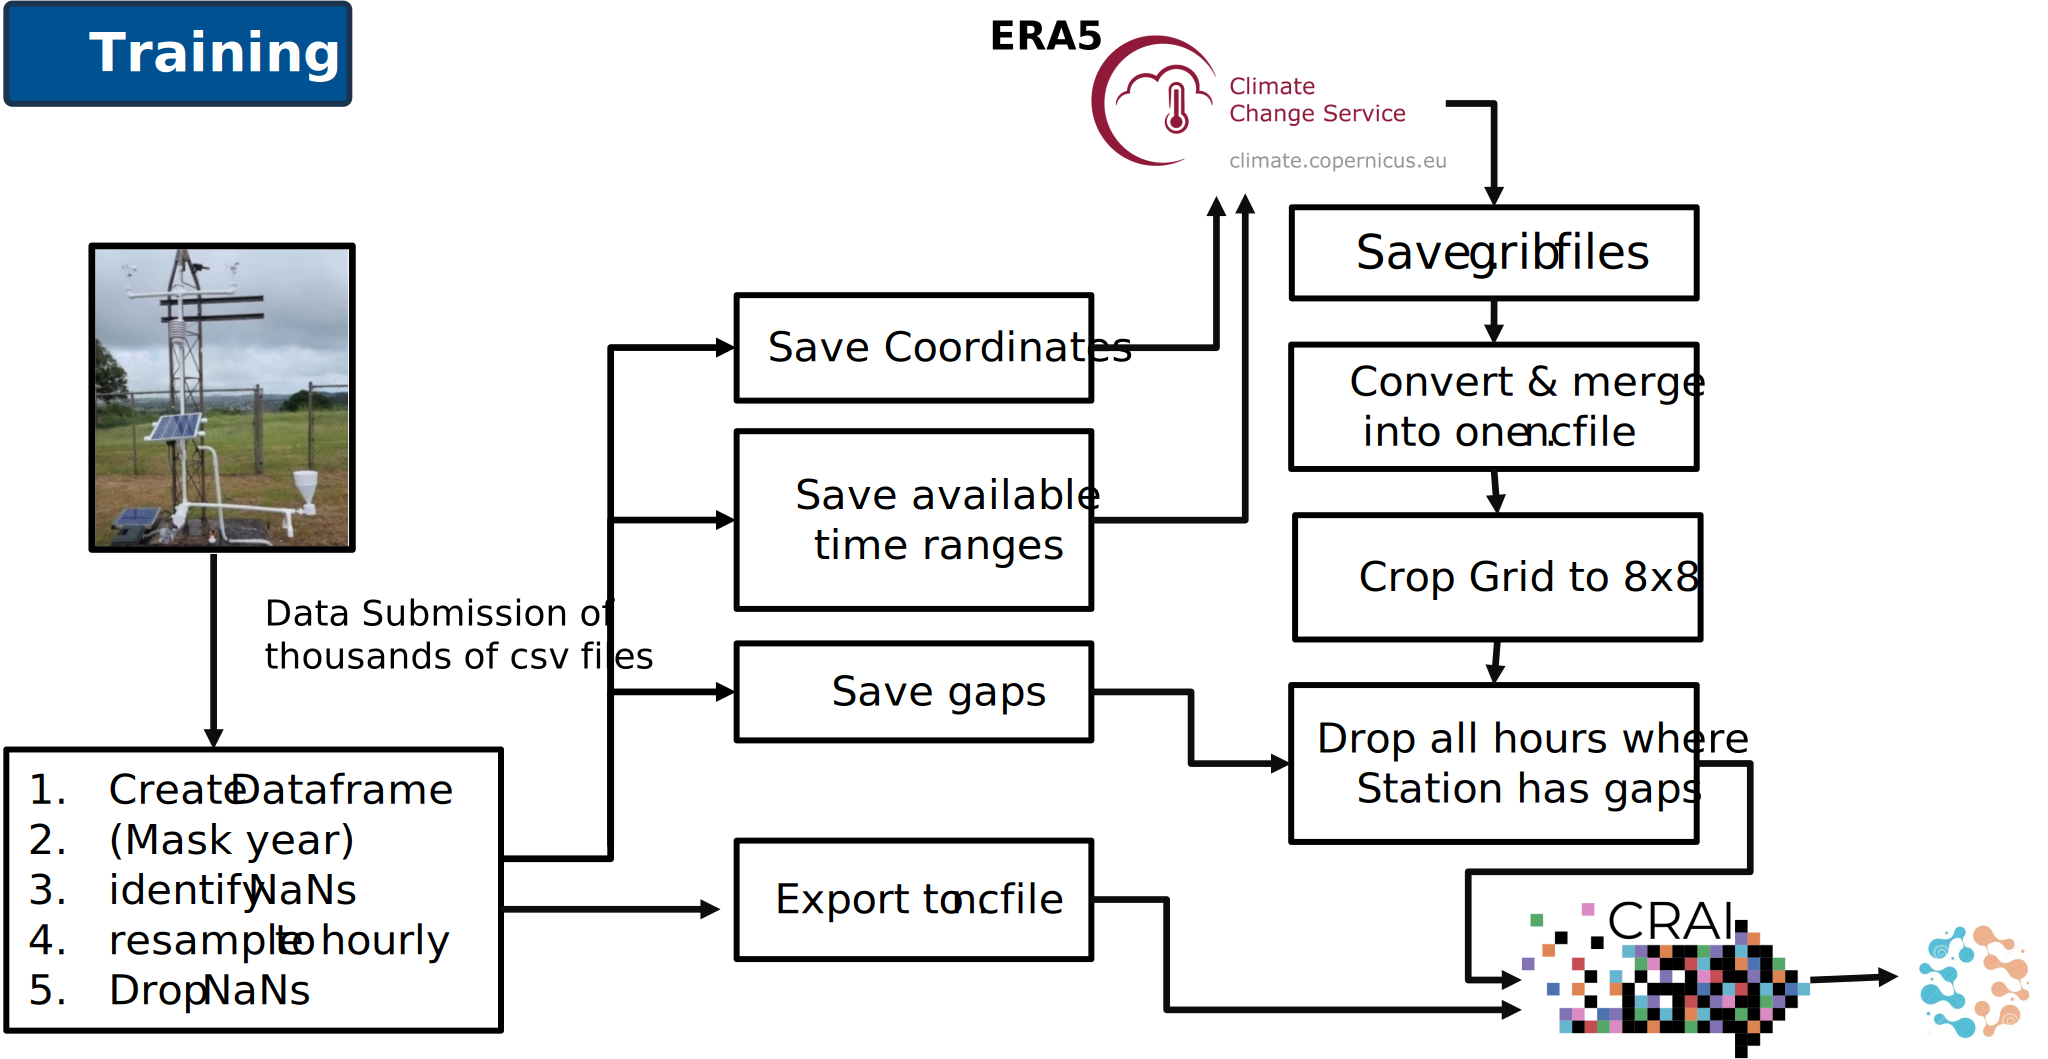
\includegraphics[width=450pt]{resources/images/training_pipeline.png}
    \caption{Pipeline to train a model}
    \label{fig: training_pipeline}
\end{figure}

\begin{figure}
    \centering
    \includegraphics[width=450pt]{resources/images/infilling_pipeline.png}
    \caption{Pipeline to reconstruct weather data using a model}
    \label{fig: infilling_pipeline}
\end{figure}

\subsection{Station Data Submission \& Conversion}

The station data for the 3D printed weather stations provided by NCAR comes in delimited text files, with one file per day, and a text-based metadata file holding information such as the station name, latitude, longitude, and elevation. 
The data files (.dat files) contain one column per sensor and one row per minute.

A class \code{DatToNcConverter} is implemented with the following functionalities:

First, it takes the \code{.dat} files and the metadata file into a directory and parses them. 
Second, the data is processed, including dropping missing values, resampling to an hourly frequency, and converting from Celsius to Kelvin to match ERA5. 
This is easiest in a pandas dataframe. 
Third, it converts the data to a \code{NetCDF} file, which is the format used by the ERA5 data and the CRAI module. 
The \code{NetCDF} file is structured in a way that stores the data in a 3D array with the dimensions time, latitude, and longitude. 
The metadata is stored as global attributes in the \code{NetCDF} file. 
Fourth, it converts some dataframes back to \code{.dat} files after the reconstruction of measurements to match the original format when infilling.

The resampling to hourly frequency is the most complex use case, as it includes many design decisions. 
Missing values are marked with \code{-999.99}, so in the first step, these values are marked as \code{NaN}. 
However, the data quality is not controlled by default, and there could be values that should be marked as missing but are not. 
Thus, the NCAR consulted to mark \code{0.00} °C as \code{NaN}. 
For stations like Barbados, this wouldn't be a realistic value, but even for regions where 0°C degrees are reached often, it is unlikely to measure exactly \code{0.00}, meaning the amount of correct data lost through marking \code{0.00} as \code{NaN} is limited. 
Additionally, by agreement with the NCAR, everything above or under \code{± 45°C} is marked as \code{NaN}. 
To compensate for peaks in the data, aggregating the minutes using a median instead of a mean is a good idea; \code{numpy.median()} would return \code{NaN} if any value is \code{NaN}, while \code{numpy.nanmedian()} would ignore \code{NaN}s. 
It is best to have a custom aggregate function using \code{numpy.nanmedian()}.

For the use case of converting the data back to a \code{.dat} file, the dataframe is stored directly in the converter object as the original dataframe. Only the detection of \code{NaN}s and the aggregation to hourly values are done before, as the use case lies in the infilling task, and the reconstruction gives hourly values.
After saving the original state, any transformation of units (Celsius to Kelvin), renaming of columns and most importantly, the actual clearing of the \code{NaN}s take place.
Fundamentally, in between the first and last measurements, rows exist for all minutes, even if measurements are missing.
However, if the station had severe issues, it is possible that between the first and last record, there are even rows or files missing.
To assure that the original dataframe, where the NaNs are not supposed to be cleared, will have rows for all hours, a handy method provided by the Python pandas module is used:

\begin{lstlisting}
    self.original_df = self.original_df.reindex(
        pd.date_range(start = self.dataframe.index.min(), end = self.dataframe.index.max(), freq = "h"))
\end{lstlisting}

A class \code{Station} is implemented to hold the metadata and the pandas dataframe of the station data.
It includes the converter itself, minimizing lines of code in the main script.
The class primarily manages access to the different files and data, both before and after the conversion.
Additionally, it detects gaps in the data, providing a simple list of hours where data is missing for infilling purposes.
For training use cases, it also lists the months where at least some data is available, which is convenient when using the API to obtain ERA5 data for the station.


\begin{lstlisting}[caption=Gap Detection in Station Class, label=lst:find_gaps]
def find_gaps(self) -> None:
available_hour_steps = self.df.index
all_hour_steps = self.converter.original_df.index
# find all hours between the first and last hour that are missing
missing_hours = all_hour_steps.difference(available_hour_steps)
return missing_hours.tolist()
\end{lstlisting}

\begin{lstlisting}[caption=Detection of available ranges in Station Class, label=lst:available_ranges]
def get_all_months_in_df(self) -> None:
# return all (year, month) tuples in the dataframe
periods = self.df.index.to_period('M').unique().tolist()
month_dict = {}
for period in periods:
    if period.year not in month_dict:
        month_dict[period.year] = []
    month_dict[period.year].append(period.month)
return month_dict
\end{lstlisting}

\subsection{Copernicus Climate Data Store - CDS API}
\label{sec: cds_api}

The Copernicus Climate Data Store (CDS) is a service by the European Centre for Medium-Range Weather Forecasts (ECMWF).
The CDS API provides open source access to the ERA5 data, allowing users to download the data for a specific location and time period.
After creating an account online an API Key can be obtained for free and with the python module 'cdsapi' data can be downloaded then easily in .grib format. 

\begin{lstlisting}[caption=Download Hook for ERA5 Data, label=lst:download_hook]
import cdsapi

class Era5DownloadHook:
    
    def __init__(self, lat, lon):
        self.cds = cdsapi.Client(
            url="https://cds.climate.copernicus.eu/api/v2",
            key=f"{os.getenv('UID')}:{os.getenv('API_KEY')}"
        )
        self.lon, self.lat = lon, lat

    def _download(cds, date_info, save_to_file_path):
        cds.retrieve(
        'reanalysis-era5-single-levels',
        {
            "product_type": "reanalysis",
            "format": "grib",
            "variable": "2m_temperature",
            "area": [
                self.lat + 1, # limit north
                self.lon - 1 % 360, # limit west
                self.lat - 1, # limit south
                self.lon + 1 % 360, # limit east
            ],
            "year": date_info.get("years"),
            "month": [f"{month:02d}" for month in date_info.get("months")],
            "day": [f"{day:02d}" for day in date_info.get("days")],
            "time": [f"{hour:02d}:00" for hour in date_info.get("hours")]

        }, save_to_file_path)



\end{lstlisting}

As seen in the code snippet, the request needs to include besides basic informations such as variable / format / model, the regional selection and the selection in the time dimension.
to download a few hours in a day the following can be used.
When building requests that download a month or a full year, it becomes obvious why the \autoref{lst:available_ranges} is so useful.

\begin{lstlisting}[caption=Download Hours in Same Day in Download Hook Class, label=lst:download_hours_in_same_day]
    def download_hours_in_same_day(self, year, month, day, hours, target_folder):
        self.download({
            "years": [year],
            "months": [month],
            "days": [day],
            "hours": hours
        }, f"{year}_{month}_{day}.grib")
\end{lstlisting}

In the \autoref{lst:download_hook} it can be seen that the regional selection is always +/- 1 degree around the Station location.
This ensures because of the grid interval of 0.25° that the downloaded area always includes at least 9x9 grid points, such that when cropping to an 8x8 selection the station can always be centered, even without exact knowledge of the coordinates of the desired grid points prior requesting. 


\subsection{Data Preprocessing}

As pointed out in \autoref{sec: cds_api} the data is downloaded in .grib format. Using the program 'cdo' the data can be quickly converted to \code{.nc} format.
With the following simple command

\begin{lstlisting}
cdo -f nc copy {source_path} {nc_path}
\end{lstlisting}

However to have the temperature at surface variable name unified as \code{"tas"} in the \code{NetCDF} file, the following command can be used:

\begin{lstlisting}[caption=Renaming Variable in \code{NetCDF} File, label=lst:rename_variable]
    import xarray as xr
    import subprocess

    def _rename_variable(self, var_name, tas_name, input, output):
        rename_variable_command = \
            f"cdo chname,{var_name},{tas_name} {input_path} {output_path}"
        subprocess.run(rename_variable_command, shell=True)
        
    ds = xr.open_dataset(input_path)
    if 'var167' in ds.variables:
        _rename_variable('var167', 'tas', input_path, output_path)
    elif '2t' in ds.variables:
        _rename_variable('2t', 'tas', input_path, output_path)

\end{lstlisting}

Then the files are merged using 

\begin{lstlisting}
    cdo cat {temp_dir_path}/*.nc {era5_target_file_path}
\end{lstlisting}

before the data is cropped to the 8x8 grid around the station location, as described in \Ref{subsec: data_preprocessing}.

For training the data it needs to be assured that the ERA5 data does not include timesteps that the nc file of the station data does not include so that the time dimensions are identical.
This is done in two steps, first the ERA5 data is cropped using a start / end date approach using the first and last date of the station data.
Then all hours that were missing in the station dataset, identified by the find gaps method in \autoref{lst:find_gaps}, are removed from the ERA5 data.
This is done using the python module xarray and deleting the timesteps in batches of up to 1000 timesteps, as deleting all at once could cause issues.

The station data should have the same dimensions as the ERA5 data, so a method is applied that coppies the ERA5 dataset and replaces all the temperature values with the measured value from the corresponding hour in the station data.

For evaluating the model, in a validation procedure the same preparation of ERA5 data is done, however instead of passing the station data as expected output to the model, the file will not be filled with the measured values but with \code{NaN}s.

When evaluating the model not for validation but to infill missing values, the ERA5 data needs to be prepared differently of course.
Instead of requesting monthly data from the cdsapi, it is requesting only the missing hours day by day, such that the time-dimesion is directly as desired, and preprocessing only needs to handle the conversion and geographical cropping.

\subsection{Handling the Model Output}

Because CRAI is using the encode, decode architecture as described in \autoref{subsec: cnn}, the output file in \code{NetCDF} format that the model produces includes not only one temperature value per timestep but has the same dimensions as the input ERA5 file meaning it uses the same 8x8 grid with 64 temperature values.
However since it has been trained on input files where the ground truth was also laid on the 8x8 grid, the 64 temperature values in the output data of the model tend to be extremely similar.
To make this transformation but primarily for practical reasons, the output file will be converted to a pandas dataframe again, where the calculated mean of the 64 values is stored.
There are two different methods implemented however creating different dataframes, as the model is evaluated in two different usecases.
One is the validation of the model, where the output is compared to the ground truth, and as in \autoref{sec: results} to ERA5 nearest grid point.
The other is the infilling of missing values, where the output is not compared but the original dataframe of the station data is updated with reconstructed values.
Both methods take the output file of the model as input, while the validation method also needs to take the groud truth and ERA5 into account.
For the ground truth, the file created by the \code{DatToNcConverter} is used, while for the ERA5 data the file that has been passed to the model is used.
The ground truth file still is using the coordinates of the station and is not stretched to the 8x8 grid, as it had been done in the training.
Therefore the method to create the validation dataframe \code{era5\_vs\_reconstructed\_comparision\_to\_df} can obtain the station coordinates from that file, and then decide which grid point in the ERA5 data is the nearest to the station.
To highlight one last core method, \code{plot\_n\_steps\_of\_df} is very useful during validation and powered the standardized plotting of the results (\autoref{fig: validation_results}).
It takes in the dataframe, returned by \code{era5\_vs\_reconstructed\_comparision\_to\_df}, and plots the temperature values of the station, the ERA5 nearest grid point, and the reconstructed values for a specific number of timesteps.
One handy feature is that if a number of timesteps is given it will plot the only that amount of timesteps, allowing for a more detailed view of the results.
It chooses the extract of \code{n} consecutive timesteps randomly, leading to the weekly extract plots in \autoref{fig: validation_results}.
In all the created plots in \autoref{fig: validation_results} the RMSE and the correlation coefficient are calculated and displayed in the title of the plot,
that has also been done in the method \code{plot\_n\_steps\_of\_df}.
Lastly, the method is also able to plot the temperature differentials instead of the absolute values, when told to do so by an optional boolean flag.
It offsets the values of course after the calculation of the RMSE and correlation coefficient.
In all these functionalities, the plotting method heavily benefits from the creation of the dataframe, as it can slice along the time dimension conveniently.

\section{Process Orchestration + API \& Webinterface}
\label{sec:process_orchestration}
\subsection{Executer Classes: Training, Infilling, Validation}


\subsection{Webinterface}

\begin{wrapfigure}[11]{r}{0.5\textwidth}
    \centering
    \includegraphics[width=0.5\textwidth]{resources/images/webinterface_screenshot.png}
    \caption{Screenshot of the webinterface}
    \label{fig:webinterface_screenshot}
\end{wrapfigure}

As written in the Introduction of this chapter, the benefit of establishing the abstraction layer with the executor classes is that with minimal additional effort, API Endpoints for initiation of processes to train/validate a model as well as endpoints to retrieve the results after the processes have finished. Additionally, it is possible to monitor the progress of the process through the API. The details on the API are described in \autoref{sec:api} This lays out a sufficient foundation for the implementation of a web interface, which is the main focus of this section.

The interface consists of two areas, one where the user is supposed to submit a "dataset", which in this context is meant as a collection of measurements from a weather station and the station's information such as location, and optionally a custom name and third a trained model for the station that can be provided optionally as well. If no model is provided the system can train a model and will attach it. 

The second area is a list of all datasets that the user has submitted. The API implementation allows for user identification through a unique token that is passed on to the server when the user submits a dataset, such that the user can then ask to see all datasets owned by them using that same token. The web interface automatically generates a token for the user and stores it then in the local storage of the browser, such that the user does not have to remember it.

As examples in \autoref{fig:webinterface_screenshot} show each dataset depending on its state has different options available. The deletion and train buttons all have in common, as no model is necessary to train a model. Datasets where a model has been provided still could be used to train a new model overwriting the old one. The "Evaluate" and "Fill in" buttons to evaluate the model over the timesteps where measurements are available, respectively to evaluate the model over the timesteps where measurements are missing.

Once a process such as training evaluation or infilling has been completed for a dataset the user can download the results anytime through the new buttons that appear in the dataset list. For example, it can be seen in \autoref{fig:webinterface_screenshot} that for the Vienna example, validation has been completed, and the user can now download a PDF with all the plots that compare the predictions with the actual measurements, or a CSV file with the same data, or a zip file that contains both and the images used in the PDF. The first Barbados example has a model attached that can be downloaded, meaning either it was provided or generated through training on the server itself. The second Barbados example has no model attached yet, meaning only the buttons "Train" and "Delete" are available, because no model was provided and no training has been done yet. 


\subsection{API Endpoints}
\label{sec:api}

% POST /data-submission
\subsubsection*{POST /data-submission}

% - GET /available-datasets/<cookie>
\subsubsection*{GET /available-datasets/<cookie>}

% - GET /train/<data-submission-id>
\subsubsection*{GET /train/<data-submission-id>}

% - GET /validate-model/<dataset-id>
\subsubsection*{GET /validate-model/<dataset-id>}

% - GET /fill-in/<dataset-id>
\subsubsection*{GET /fill-in/<dataset-id>}

% - DELETE /delete-dataset/<dataset-id>
\subsubsection*{DELETE /delete-dataset/<dataset-id>}

% - GET /download-model/<dataset-id>
\subsubsection*{GET /download-model/<dataset-id>}

% - GET /download-validation-zip/<dataset-id> (just pdf and csv available too)
\subsubsection*{GET /download-validation-zip/<dataset-id>}

% - GET /download-infilling/<dataset-id>
\subsubsection*{GET /download-infilling/<dataset-id>}

\section{Conclusion}
\label{sec: discussion}

% \subsection{2 step process}
\subsection{Outlook \& Improve quality}

\subsection{Possible applicances}
% \subsection{Use for weather forecasting}


% Bibliografie im .bib Format einfügen

\bibliography{references}

\end{document}
